\section{Implementation}
\label{sec:implementation}

\subsection{Landslide}
\label{sec:landslide}

We chose \landslide~\cite{landslide} as our stateless model checker due to its ability to trace program execution at the granularity of individual instructions and memory accesses, which dynamic data-race detection requires.
\landslide~implements DPOR \cite{dpor},
%\cite{dpor},
state space estimation \cite{estimation}, and a hybrid lockset/happens-before data-race analysis \cite{hybriddatarace}.
% TODO: \cite{fairstatelessmc} instead or in addition?
It avoids state space cycles (e.g. ad-hoc synchronization with {\tt yield()} or even {\tt xchg} loops) with a heuristic similar to Fair-Bounded Search \cite{bpor}.
% this line can be cut if space is needed
It can test both user-level and kernel-level code, although is limited to timer-driven nondeterminism.
% joshua wants "segfault" to be "memory access error (i.e., segmentation fault, or bus error)"
Its bug-detection metrics include assertion failure, deadlock, segfault, heap checking (like Valgrind~\cite{valgrind}), and a heuristic infinite loop/livelock check.

{\bf Restricting PPs with stack trace predicates.}
Most model checkers (MCs) preempt indiscriminately on any sync API call, regardless of the call-site.
However, when testing a particular module in a large codebase,
the user is likely uninterested in PPs arising from other modules.
\landslide~provides the {\tt within\_function} configuration command for a user to identify which call-sites matter most.
Before inserting a PP, \landslide~requires at least one argument to {\tt within\_function} to appear in the current thread's stack trace.
%The {\tt without\_function} directive works similarly, but as a blacklist.
The {\tt without\_function} directive is the dual of {\tt within\_function}, indicating a blacklist.
Multiple invocations can be used; later ones take precedence.
%\cite{landslide} provides further detail on this feature.

{\bf Data races in lock implementations.}
Data race tools in prior work \cite{tsan,portend} recognize the implementations of sync primitives to avoid spuriously flagging memory accesses resulting from the lock implementation itself.
The assumption that the locks are already correct enables productive data-race analysis on the rest of the codebase.
Otherwise, with testing limited to one execution,
%even if one wishes to test for lock bugs,
data-race analysis would flag every access pair in the lock implementation, requiring human attention to verify.
However, Iterative Deepening can automatically verify a large quantity of data-race candidates as benign.
Hence, we extended \landslide~with a custom option to change the lock-set tracking to include accesses from {\tt mutex\_lock()} and {\tt mutex\_unlock()} in the analysis. (Accesses from other sync functions, such as {\tt cond\_wait()}, would either be included already, or be protected by an internal mutex.)

\subsection{Quicksand}

\quicksand~is an independent program that wraps the execution of several \landslide~instances.
The implementation is roughly 3000 lines of C.
It uses a thread pool to schedule the available state spaces,
sorting such jobs according to their status among a running queue, pending queue, and suspended queue.
Jobs are further prioritized by number of PPs, ETA, and whether they include data-race PPs.

{\bf Initial PPs.}
For testing user-space code, we seed the exploration with the four subsets of ``hard-coded'' locking API PPs that we showed in Figure~\ref{fig:id}:
$\{yield\}$,
$\{yield,lock\}$,
$\{yield,unlock\}$,
and $\{yield,lock,unlock\}$,
By extension, these also introduce preemptions on any other sync primitives implemented with mutexes,
such as condition variables, semaphores, and r/w locks.
Preempting on voluntary switches such as {\tt yield} is always necessary to maintain the invariant that only one thread runs between consecutive PPs.
%so the {\tt yield} PP is always implicitly enabled.

For kernel-level testing, we consider interrupt-disabling to be analogous to locking,
so we also preempt just before a disable-interrupt opcode ({\tt cli}) and just after interrupts are re-enabled ({\tt sti})\footnote{
%(to appropriate the names of the x86 instructions)
During data-race detection, {\tt cli}/{\tt sti} are treated as a single global lock.
%as {\tt cli}'d memory accesses can still race with others that have interrupts on.
Some kernels disable preemption without disabling interrupts,
which can be modelled the same way using manual annotations. %of that API.
This also assumes uni-processor scheduling; for SMP kernels, replace {\tt cli}/{\tt sti} with spinlocks.}.
\quicksand~is configured to begin with the subsets
$\{yield\}$,
$\{yield,lock\}$,
$\{yield,unlock\}$,
$\{yield,cli\}$,
$\{yield,sti\}$,
and $\{yield,lock,$ $unlock,cli,sti\}$.
As a heuristic, we don't bother with every intermediate subset such as $\{lock,sti\}$,
which could potentially be improved in future work (\sect{\ref{sec:future}}).

{\bf Communication protocol.}
The interface to \landslide~, which any similar MC could implement, has two parts.
First, when starting each job, \quicksand~creates a configuration file declaring which PPs to use,
% can lose this line due to space
among other options such as mutex-testing mode,
passed as an argument to \landslide.
Then, a dedicated \quicksand~thread communicates with the \landslide~process via message-passing. %on a FIFO pipe.
\landslide~messages \quicksand~after testing each new interleaving to report updated progress and ETA,
whenever a new data-race candidate is found, and whenever a bug is found.
\quicksand~in turn replies whether the test should suspend/resume due to too high ETA, or quit due to timeout.
We implement suspending jobs simply by making \landslide~wait on a message-passing call.
Should \quicksand~later resume a suspended job, we send a message to continue,
causing the \landslide~instance to resume exploring where it left off;
otherwise, we send a message only after time runs out, causing it to exit.

{\bf Heuristics.}
% List of all heuristix:
% HOMESTRETCH - last 60sec of test, don't suspend
% ETA_THRESH - "to let its ETA stabilize"
% eta factor
% shold_reproduce -- small dr jobs are not allowed to add further instances of themself (why not? don't remember)
% priority change between suspected and confirmed dr
Algorithm~\ref{alg:shouldworkblock} allows heuristically scaling a job's ETA when comparing to the time budget,
to express how optimistic we are about the estimate's accuracy.
We use 2 as this scaling factor based on the results in \cite{estimation},
though we allow changing it via the command line.
We also include a heuristic to
%ignore ETAs entirely
never suspend jobs before they pass a certain threshold of interleavings tested,
for which we choose 32,
so that their ETAs have some time to stabilize.

We classify data-race candidates as {\em single-order} or {\em both-order} \cite{portend}
based on whether the MC observed the racing instructions ordered one or both ways in the original state space,
Jobs with both-order data-race PPs are prioritized higher,
because single-order candidates are more likely to be false-positives
(though before preempting during the access itself, we cannot say for sure, hence the heuristic).
%so we prioritize jobs with both-order data-race PPs.
For single-order races, we do not add a PP for the later access at all;
should it be needed, preempting on the first access will suffice to upgrade the race to both-order.

% If there's room, mention the cant_swap mechanism for killing the top half of deferred jobs.

\subsection{Data-race preemption points}

When \landslide~detects a data race, it reports each of the two memory accesses involved in the race.
Each report indicates the program counter value (PC) associated with the access, as well as some further conditions to help filter away unrelated executions of the same instruction on different data.
(For example, many parts of a codebase might call {\tt list\_insert()}, but only one callsite does so without adequate locking.)
Ideally, the PC would be qualified by a full backtrace, but tracing the stack is too expensive to do for each shared memory access.
Instead, \landslide~qualifies the PC with
(a) the current thread ID and
% FIXME: We don't actually do this.
(b) the most recent {\tt call} instruction.
% (a crude approximation of a stack trace)
% which are much cheaper, as we carry them around all the time already
Note that we do {\em not} qualify data races by the shared memory address,
which can change based on different interleavings of previous code
(for example, depending on the result of {\tt malloc()}).
% especially when malloc is involved.
%Figure~\ref{fig:dont-filter-dr-by-address} shows example code where qualifying by memory address will miss the bug.

\begin{figure}[t]
	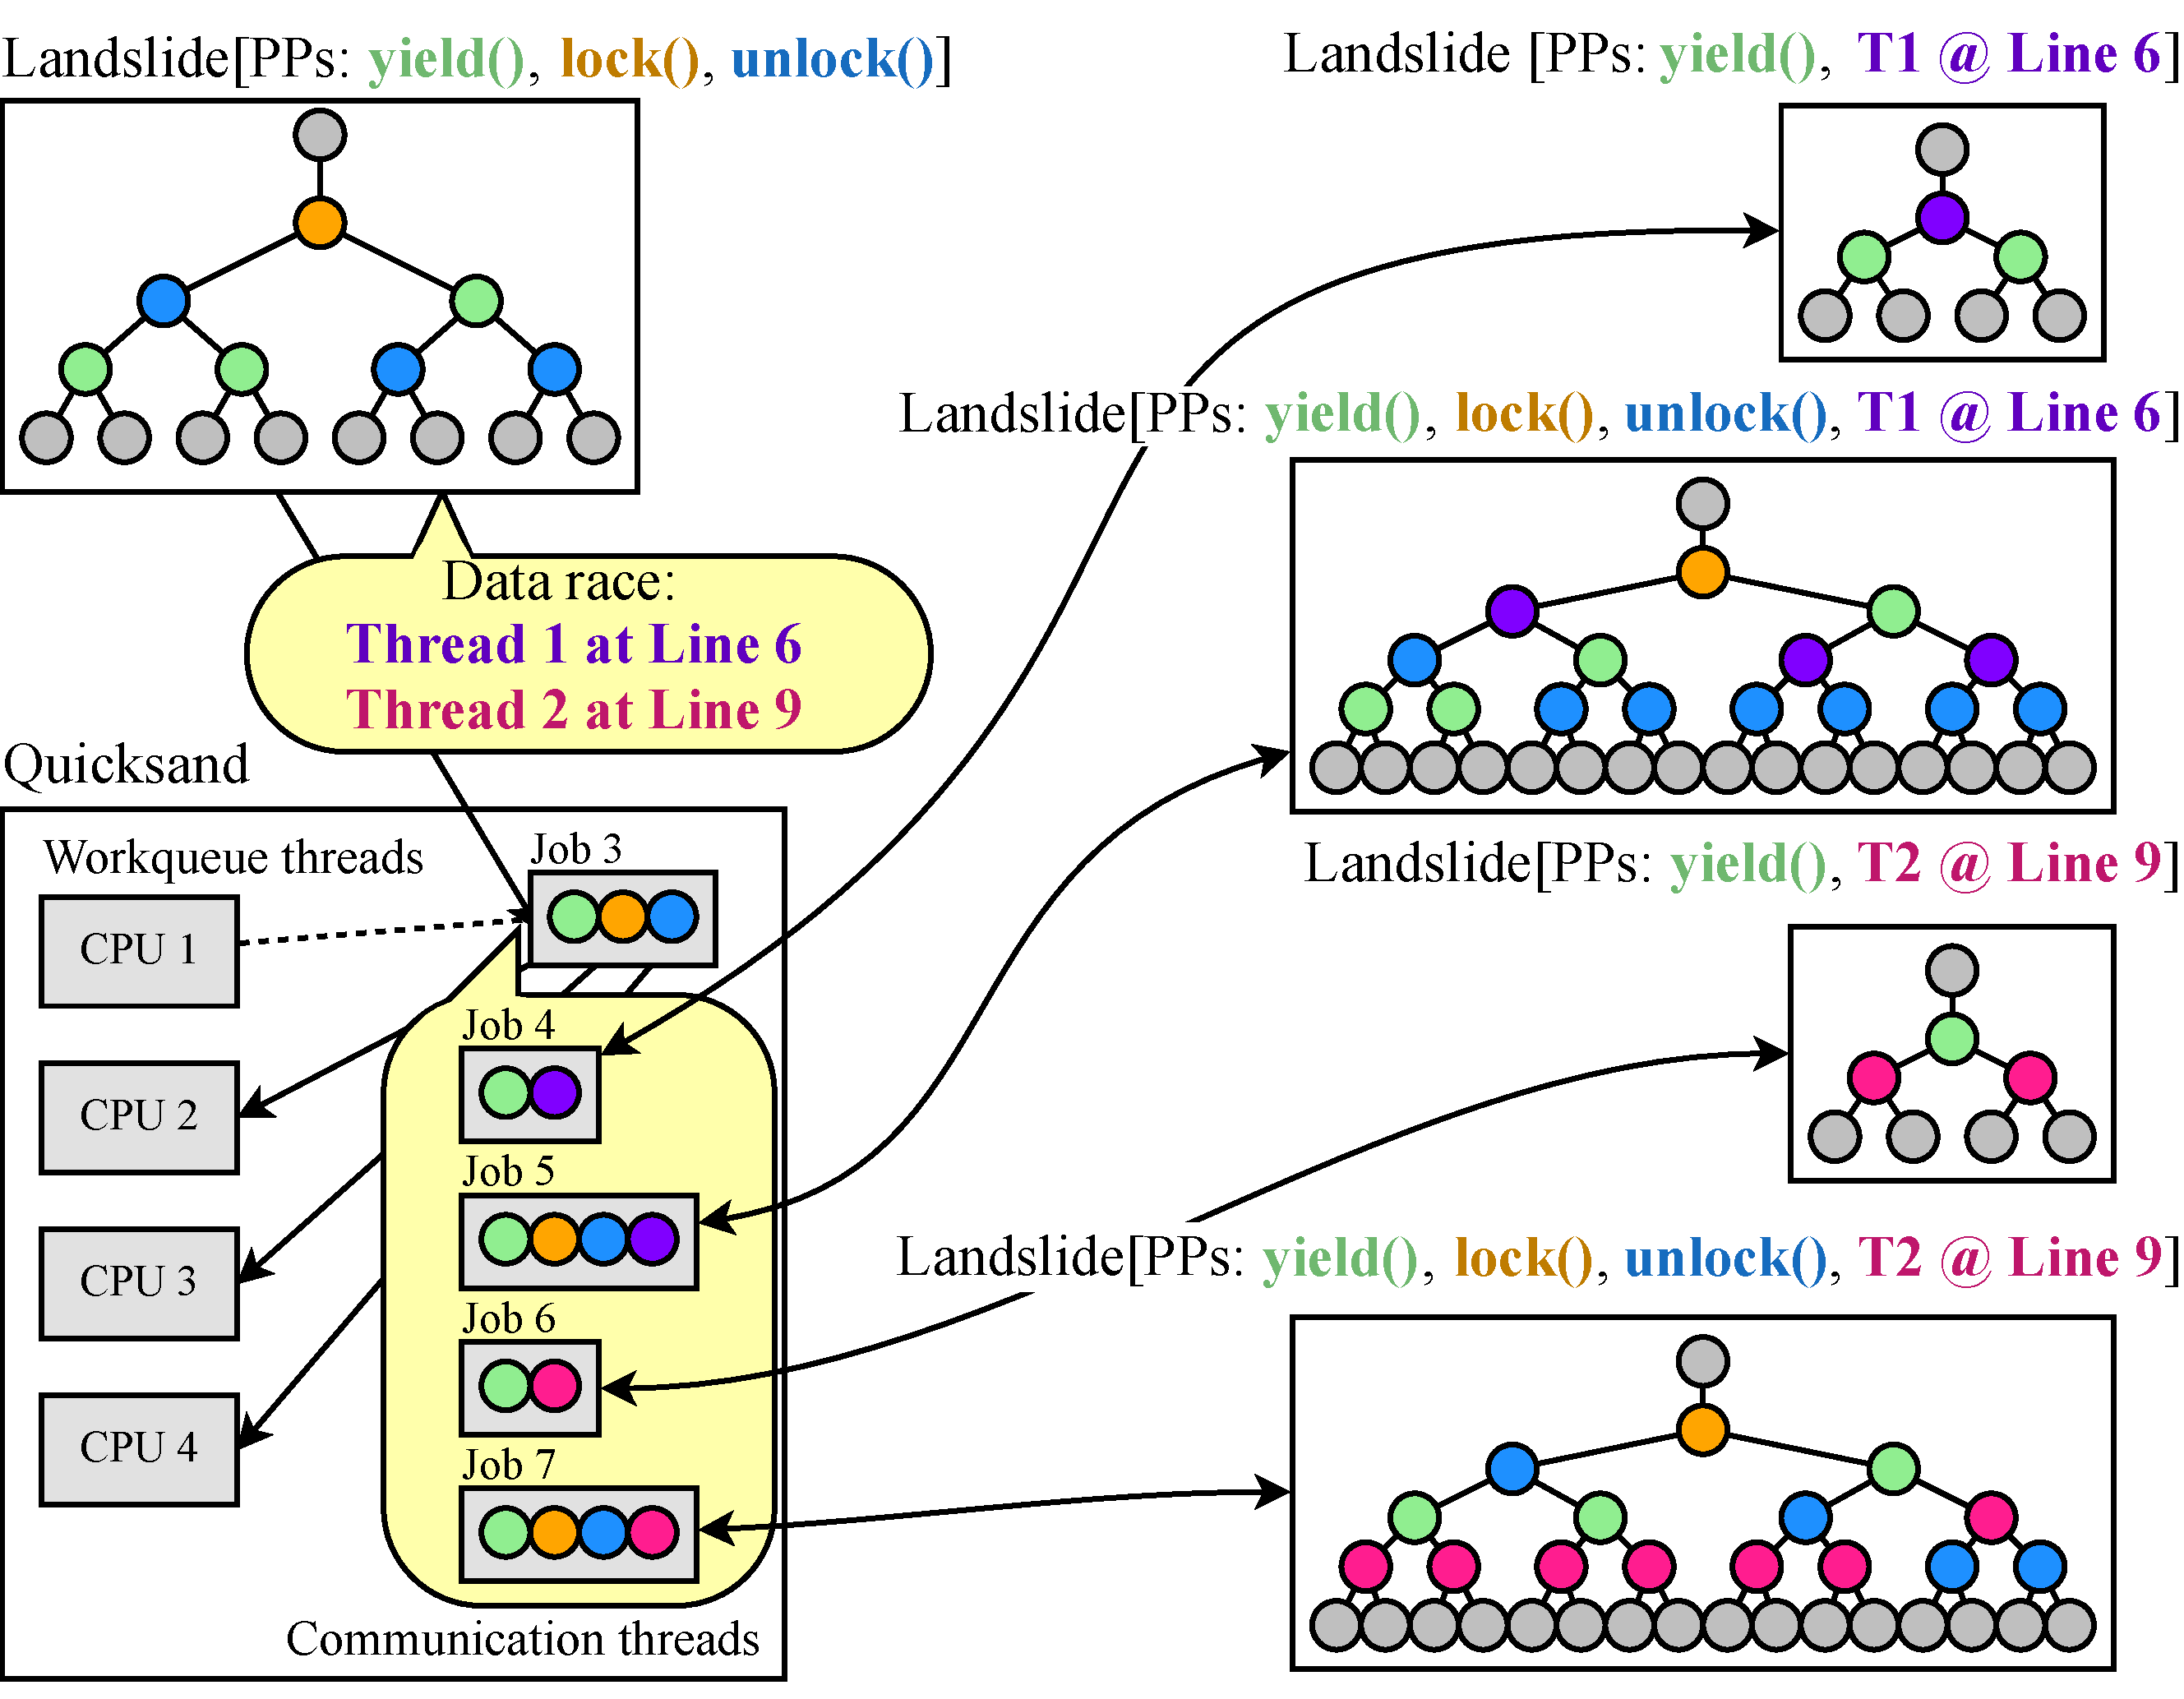
\includegraphics[width=0.48\textwidth]{dr-jobs-v2.pdf}
	\caption{\quicksand~manages the exploration of multiple state spaces, communicating with each MC instance to receive ETAs, data race candidates, and bug reports.
		When an access pair is reported as a data race, we generate a new PP for each access and add new jobs corresponding to different combinations of those with the existing PPs.}
	\label{fig:new-dr-jobs}
\end{figure}


When \quicksand~receives a data race report, it adds two new jobs to its workqueue:
a ``small'' job to preempt on the racing instruction only,
and a ``big'' job to preempt on that instruction as well as each PP used by the reporting job.
%
Hence, together with the logic in \sect{\ref{sec:classifying}}, each {\em pair} of racing accesses will spawn four new jobs, as shown in Figure~\ref{fig:new-dr-jobs}.
%
The rationale of spawning multiple jobs is that which will be more fruitful cannot be known in advance:
while the big job risks not completing in time,
the small job risks missing the data race entirely if the original PPs were required to expose it.
In practice, we observed some bugs found quickly by these small jobs, and other bugs missed by the small jobs found eventually by the big jobs,
which motivates the need for Iterative Deepening to prioritize the jobs at runtime.
% TODO: Put numbers here.

